% arara: pdflatex
% !arara: biber
% !arara: pdflatex
% How to run: 
% 1) pdflatex "filename".tex
% 2) biber "filename"
% 3) pdflatex "filename".tex
% 4) pdflatex "filename".tex


\documentclass[x11names]{article}
\usepackage{verbatim}
\usepackage{listings}
\usepackage{graphicx}
\usepackage{a4wide}
\usepackage{color}
\usepackage{amsmath}
\usepackage{amssymb}
\usepackage[dvips]{epsfig}
\usepackage[T1]{fontenc}
% \usepackage{cite} % [2,3,4] --> [2--4]
\usepackage{shadow}
\usepackage{hyperref}
\usepackage{physics}
\usepackage{url}
\usepackage{tikz}
\usepackage{subcaption}
\usepackage[utf8]{inputenc}
\usepackage{booktabs} % Allows the use of \toprule, \midrule and \bottomrule in tables
\usepackage[font={small,it}]{caption}
\usepackage[margin=0.7in]{geometry} %Sets the margins in the document
\usepackage{siunitx}    %Allows use of SI units macros

%Defines calculator way to write powers of ten
\sisetup{output-exponent-marker=\textsc{e}}


% Change numbering and some commands
\renewcommand\thesection{Exercise \Roman{section}}
\renewcommand\thesubsection{\Roman{section}.\alph{subsection}}

%% references
\usepackage[style=authoryear,
            bibstyle=authoryear,
            backend=biber,
            % refsection=chapter,
            maxbibnames=99,
            maxnames=2,
            firstinits=true,
            uniquename=init,
            natbib=true,
            dashed=false]{biblatex}

\addbibresource{bibliography.bib}
% \addbibresource{top.bib}

% \bibliography{bibliography}
% \bibliography{top}


\usepackage[capitalize]{cleveref}

\setcounter{tocdepth}{2}

\lstset{language=c++}
\lstset{alsolanguage=[90]Fortran}
\lstset{basicstyle=\small}
\lstset{backgroundcolor=\color{white}}
\lstset{frame=single}
\lstset{stringstyle=\ttfamily}
\lstset{keywordstyle=\color{red}\bfseries}
\lstset{commentstyle=\itshape\color{blue}}
\lstset{showspaces=false}
\lstset{showstringspaces=false}
\lstset{showtabs=false}
\lstset{breaklines}


\definecolor{keywords}{RGB}{255,0,90}
      \definecolor{comments}{RGB}{0,0,113}
      \definecolor{red}{RGB}{160,0,0}
      \definecolor{green}{RGB}{0,150,0}
       
      \lstset{language=Python, 
              basicstyle=\ttfamily\small, 
              keywordstyle=\color{keywords},
              commentstyle=\color{comments},
              stringstyle=\color{red},
              showstringspaces=false,
              identifierstyle=\color{green}
              }



\title{ Exercise 2 \\ Sommerjobb Numeriske Plasmaoppgaver }
\author{Gullik Vetvik Killie
		}


%%%%%%%%%%%%%%%%%%%%%%%%%%%%%%%%%%%%%%%%%%%%%%%%%%%%%%%%%%%%%%%%%%%%%%%%%%%%%%%%%%%%
% Actual text starts here
%%%%%%%%%%%%%%%%%%%%%%%%%%%%%%%%%%%%%%%%%%%%%%%%%%%%%%%%%%%%%%%%%%%%%%%%%%%%%%%%%%%%
\begin{document}


\maketitle

\section{Exercise}

\subsection{Theory}
      \subsubsection{Equation of motion and Euler's algorithm}
      This exercise is about the trajectory of charged particles in static Electric and Magnetic external fields and as usual we start with the equation of motion for a particle and use Euler's method to to integrate calculate the trajectories. We also show that there is a constant drift velocity in the particles center of motion and compare the theoretical drift velocity with the drift velocity detected in the simulation. The equation of motion is the following

      \begin{align}
            m\pdv{\va{v}(t)}{t} &= q \left( \va{E} +   \va{v}\cross \va{B_0} \right); \qquad{} \va{E} = (E_x,E_y,0) \qquad{} \text{and} \qquad{} \va{B_0} = (0,0,B_0)
            \intertext{Using Euler's method to approximate the derivative, \( \pdv{f(t)}{t} \approx \frac{f(t+h) - f(t) }{h}\), we arrive at }
            \va{v}(t + h) &= \va{v}(t) + h\frac{q}{m}\left( \va{E} +   \va{v}\cross \va{B_0} \right)
            \intertext{Decomposing into \(x\), $y$ and $z$ coordinates}
            v_x(t +h) &= v_x(t) + h\frac{q}{m}\left( E_x +   v_yB_0 \right)
            \\
            v_y(t + h) &= v_y(t) + h\frac{q}{m}\left( E_y -   v_x B_0 \right)
            \\
            v_z(t + h) & = v_z(t) + h\frac{q}{m}\left( E_y \right)
      \end{align}
      We only need to concern ourselves with the \(x\)- and \(y\)- coordinates since the \(z\) velocity is constant with our electric field. We will use the same algorithm as in the previous exercise and it is listed below

      \begin{enumerate}
            \item Declare variables $h$, $q$, $m$, \(B_0\) and vectors \(v_x\), $v_y$, $x$, and $y$.
            \item Set initial conditions
            \item For loop until counter \(\leq\) timesteps. Update \(v_x(t+ h)\), $v_y(t+ h)$, $x(t + h)$ and $y(t + h)$.
            \item Plot and analyze results
      \end{enumerate}

      \subsubsection{E cross B drift}
      To find the theoretical drift we first decompose the velocity into a velocity along the magnetic field ,$\va{v}_\parallel $,, a perpendicular gyration velocity ,$\va{\omega}_\perp $, and a constant drift , $\va{v}_D $, and then we can solve those seperately.

      \[ \va{v} \rightarrow \va{v}_\parallel + \va{\omega}_\perp + \va{v}_D \]
      
      The equation of motion is then

      \begin{align}
           \pdv{\va{v}_\parallel}{t} + \pdv{\va{\omega}_\perp}{t} + \pdv{\va{v}_D}{t} &= \frac{q}{m} \left( \va{E}_\perp +   \left( \va{v}_\parallel + \va{\omega}_\perp + \va{v}_D \right)  \cross \va{B}_0 \right)
      \end{align}

      The parallel velocity is unaffected by the magnetic field

      \begin{align}
            \pdv{v_\parallel}{t} &= \frac{q}{m} E_\parallel
            \\
            v_\parallel &= \frac{q}{m} E_\parallel t
      \end{align}

      Then we handle the gyration velocity
      \begin{align}
            \pdv{\va{\omega}_\perp}{t} &= \frac{q}{m}\va{\omega}_\perp \cross \va{B_0}        \label{eq:gyro_vel_1}
            \intertext{Let us do a temporal derivative}
            \pdv[2]{\omega_\perp}{t} &= \frac{q}{m} \left(\pdv{\omega_\perp}{t} \cross \va{B}_0\right)
            \intertext{Let us then substitute \cref{eq:gyro_vel_1} into the equation to obtain }
            \pdv[2]{\omega_\perp}{t} &= \frac{q}{m} \left(\frac{q}{m} \va{\omega}_\perp \cross \va{B_0} \right)  \cross \va{B}_0
            \intertext{Then we use the vector relation \(a\cross b \cross c = b(a\cdot c) - c(a\cdot b)\) to get}
            \pdv[2]{\va{\omega}_\perp}{t} + \omega_c ^2 \va{\omega}_\perp&= 0
            \intertext{where \( \omega_c = \frac{q B_0}{m} \). Using that the gyration velocity magnitude is \(v_x^2 + v_y^2 = \omega_\perp\) a solution for this differential equation is}
            \va{\omega_\perp}(t) &= 
                  \begin{pmatrix}
                        \omega_\perp \cos(\frac{qB_0}{m}t + \theta)
                        \\
                        -\omega_\perp \sin(\frac{qB_0}{m}t + \theta)
                        \\
                        0
                  \end{pmatrix}
            \intertext{where \(\theta\) the phase of the gyration we are starting at.}            
      \end{align}

      \noindent Since we assumed that the drift was constant we set the time derivative to 0 when solving for the drift.

      \begin{align}
            0 &= \frac{q}{m} \left(\va{E}_\perp +  \va{v}_D \cross \va{B_0}\right)
            \intertext{Then we cross the equation with \(\va{B_0}\) and use the same vector identity as earlier to obtain}
            \va{B_0} \cross  \left(\va{v}_D \cross \va{B_0} \right) &= \va{B_0} \cross (- \va{E}_\perp)
            \\
            \va{v}_D &= \frac{\va{E}_\perp \cross \va{B_0}}{B_0^2} = \frac{1}{B_0} 
            \begin{pmatrix}
            E_x \\ E_y \\ 0
            \end{pmatrix}
      \end{align}

      The complete solution for the velocity is then, if we only take the case where \( v_z = E_z = 0 \) for simplicity

      \begin{align}
            v_x (t) &= \omega_\perp \cos(\frac{qB_0}{m}t + \theta) + \frac{E_y}{B_0}      \label{eq:vx}
            \\
            v_y (t) &= -\omega_\perp \sin(\frac{qB_0}{m}t + \theta) - \frac{E_x}{B_0}     \label{eq:vy}
      \end{align}

      Then by integrating we obtain the position of the particle

      \begin{align}
            x(t) &= x_c + \rho_c \sin(\frac{qB_0}{m}t + \theta) + \frac{E_y}{B_0}t
            \\
            x(t) &= y_c + \rho_c \cos(\frac{qB_0}{m}t + \theta) - \frac{E_x}{B_0}t
      \end{align}

      \noindent where \(x_c\) and $y_c$ is initial position of the guiding center.


\subsection{Results}
      
      \subsubsection{Trajectories of the particles}
      For the code solving the problem see \cref{sec:code}

      \begin{figure}
            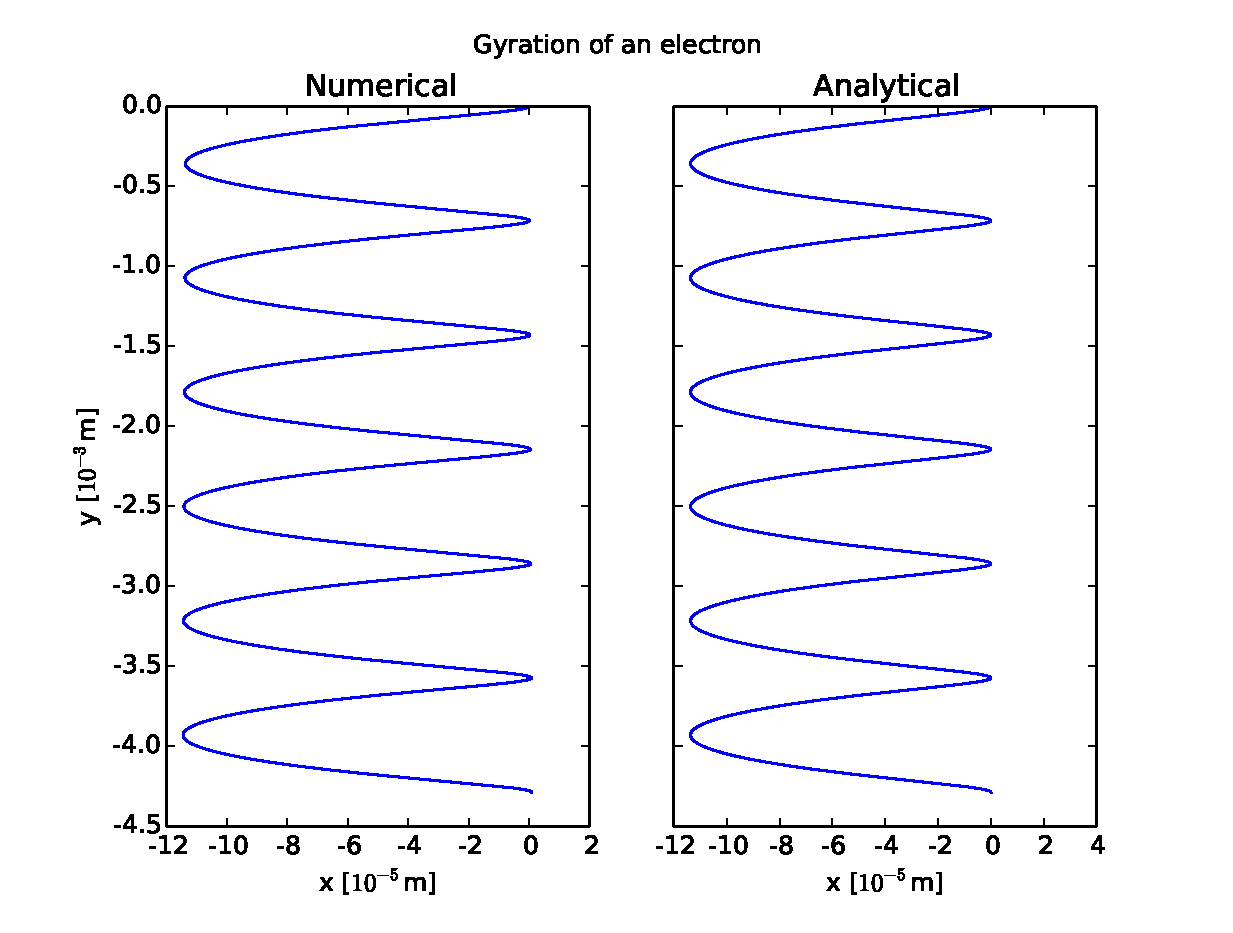
\includegraphics[width = 0.5\linewidth]{../source/ExBelectron}
            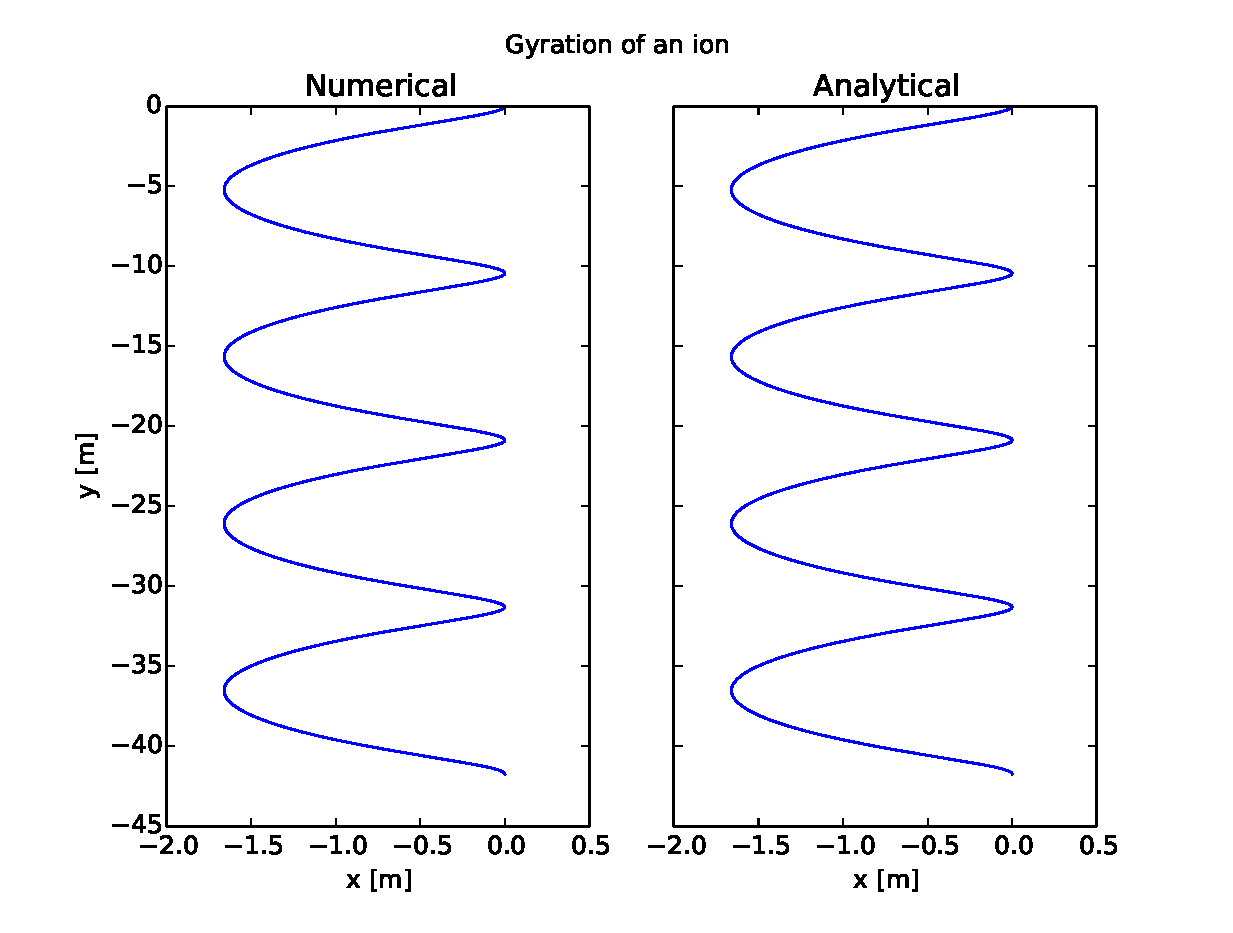
\includegraphics[width = 0.5\linewidth]{../source/ExBion}
            \caption{These plots show the trajectories of an electron and an ion in a static magnetic field, \(\va{B}_0 = (0,0,50000) \si{\nano\tesla}\), and a static electric field \( \va{E} = (50,0,0)  \si{\milli\volt\per\meter}\). The stepsize used for the electron simulation were \(10^{-10} \si{\second}\) and for the oxygen ion \(10^{-6} \si{\second}\)}
            \label{fig:ExBDrift}
      \end{figure}

      In \cref{fig:ExBDrift} we can see the trajectories to an electron and an oxygen ion in a static magnetic field and a static electric field, a new feature introduced to the trajectories compared to the earlier examined case with no electric field is a constant drift of the guiding center. We see that the direction of the drift is independent of the charge of the particle and is given perpendicular to the electric and magnetic field. In \cref{tab:drift} the drift velocity observed in the simulation is compared with the theoretical drift velocity given by \(\vb{v}_D = -\frac{E_x}{B_0}\vu{j}\).

      \begin{table}
            \centering
            \begin{tabular}{| c | c | c |}
                  \hline
                                          & Numerical $v_D$  [$10^3 \si{\meter\per\second}$]   & Theoretical $v_D$ [$10^3 \si{\meter\per\second}$]   
                  \\ \hline
                  e                       &  $1.00$   &    $1.00$ 
                  \\ \hline
                  O$^+$                   &  $1.00$  &     $1.00$ 
                  \\ \hline
            \end{tabular}
            \caption{The magnitude drift in experienced for an electron and an oxygen ion in a static magnetic and electric field. For the electron a timestep of \( 10^{-10} \si{s} \), while for the oxygen ion \( 5\times 10^{-5} \si{\second } \) long timesteps were used.}
            \label{tab:drift}
      \end{table}

      \subsubsection{Varying direction of initial velocity}
      The radius of a particles gyration is dependent on the initial conditions, as can be seen in \cref{fig:VaryVElectron} and \cref{fig:VaryVion}. If we take examine \cref{eq:vx} and \cref{eq:vy} at \(t=0\) we get 
      \begin{align}
            v_x (0) &= \omega_\perp \cos(\theta) + \frac{E_y}{B_0}      
            \\
            v_y (0) &= -\omega_\perp \sin(\theta) - \frac{E_x}{B_0}     
            \intertext{In our simulation we set the initial magnitude of the velocity to be \( v_0 = \sqrt{v_x^2 + v_y^2} = 500 \si{\meter\per\second}\), and setting \(E_y = 0\)}
            \omega_\perp^2 &= \left( v_x \right)^2 + \left( v_y + \frac{E_x}{B_0}   \right)^2 \label{eq:omega_perp}
            % \\
            % v_0^2 &= \omega_\perp^2 + 2\omega_\perp \sin(\theta) \frac{E_x}{B_0} + \left(\frac{E_x}{B_0} \right)^2
      \end{align}

      Since the gyration radius \(\rho_c = \omega_\perp / \omega_c \) the gyration radius is at a minimum when initial velocity is aligned with the E-cross-B drift, and at a maximum when it is aligned the opposite way. This can also be solved exactly.

      \begin{figure}
            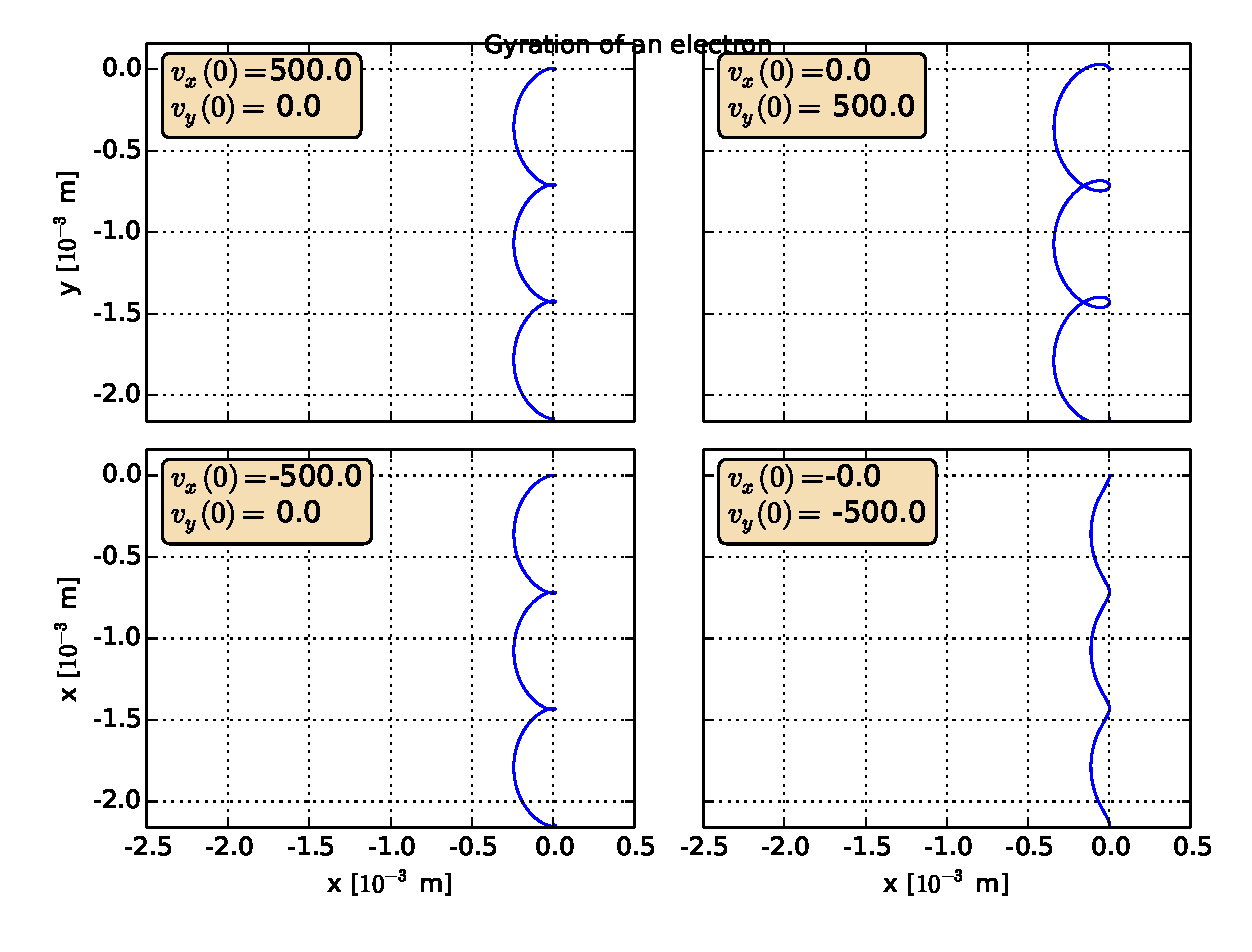
\includegraphics[width = \linewidth]{../source/ExBVaryingVelectron}
            \caption{The trajectories for an electron moving in homogenous and static electric and magnetic fields. The magnitude of the initial velocities is \(500 \si{\meter\per\second}\) but the direction is rotated \(\pi/2\) for each plot.}
            \label{fig:VaryVElectron}
      \end{figure}

      \begin{figure}
            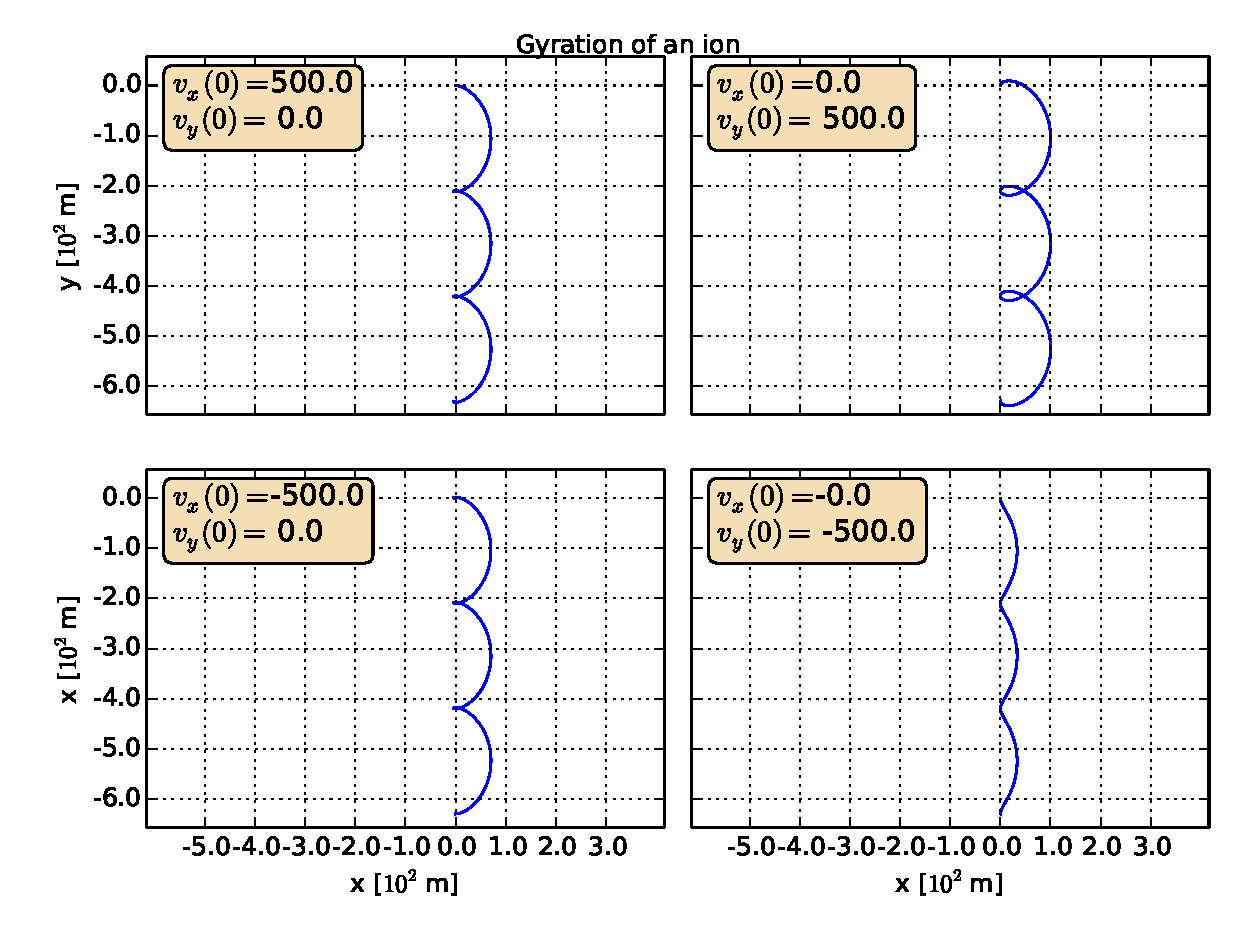
\includegraphics[width = \linewidth]{../source/ExBVaryingVion}
            \caption{The trajectories for an ion moving in homogenous and static electric and magnetic fields. The magnitude of the initial velocities is \(500 \si{\meter\per\second}\) but the direction is rotated \(\pi/2\) for each plot.}
            \label{fig:VaryVion}
      \end{figure}

\appendix

\section{Comments regarding the exercise}
      \begin{itemize}
            \item I first mistook the units of the electric field to be a typo and be \(\si{V/m}\) and the extra \(m\) to just be a typo. I realized later that it was millivolt. I think that was just on me.
            \item I had some comments about how the inital velocity should be \(\va{v}(0) = (\omega_\perp, -E_x/B_0, 0 ) =(500,-100,0) \si{\meter\per\second}\), but that was because I started to wonder why a change in the electric field changed the gyration radius. (Couldn't resist playing around) After I did part three I realized that was the entire point of what they the exercise was supposed to show. 
            \item \textit{Edit:} I see this is fixed in the second edition. \newline
            The kinetic energy is not conserved in this case, see \cref{fig:kineticEnergy}, the particle has a greater velocity when the gyration velocity is moving in the same direction as the drift velocity and a smaller when it is moving in a different direction. The gyro averaged kinetic energy (averaged over the gyration period) will be conserved though.
                  \begin{figure}
                  \centering
                        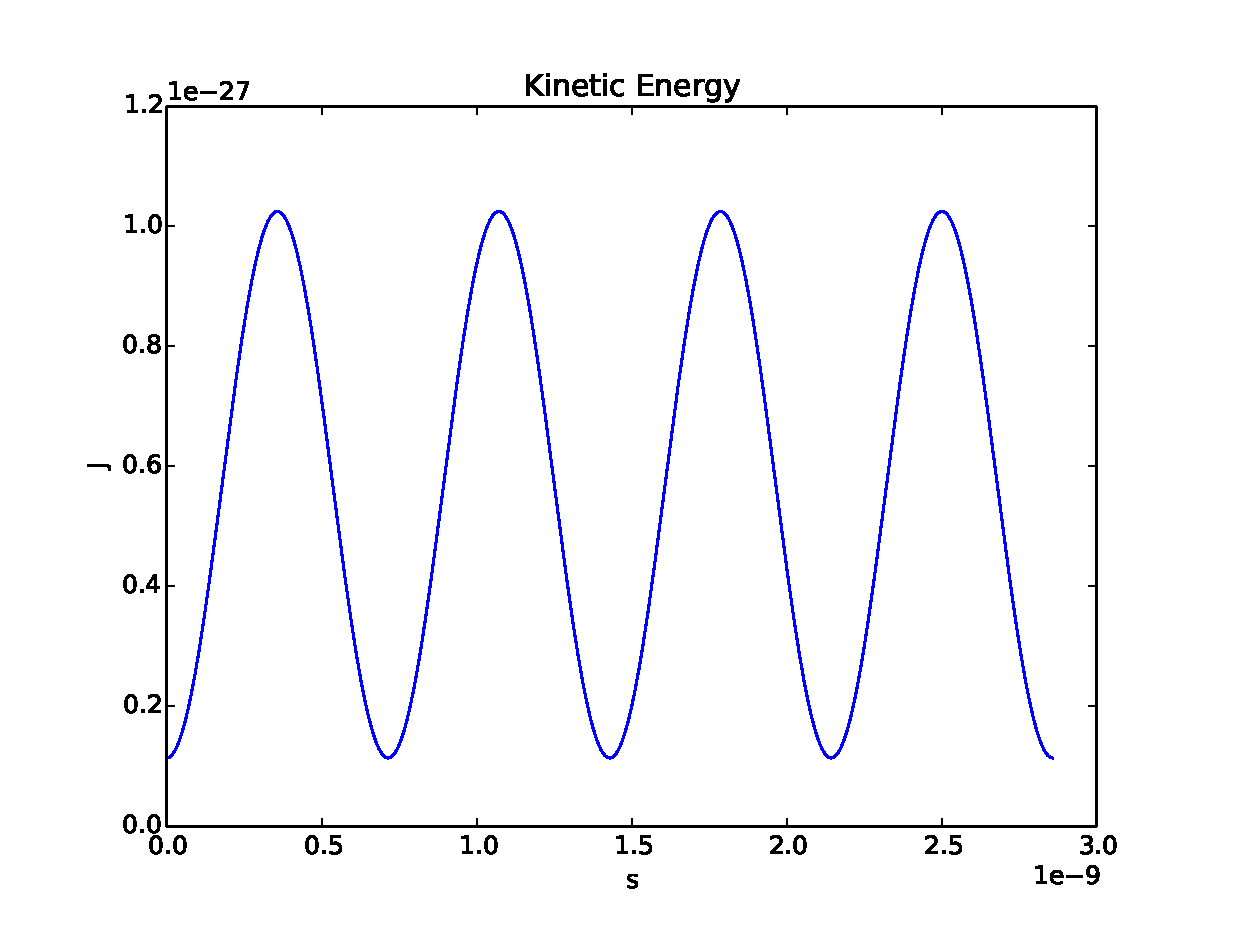
\includegraphics[width = 0.5\linewidth] {../source/kineticEnergy}
                        \caption{The Kinetic Energy of an electron moving in a static magnetic and electric field}
                        \label{fig:kineticEnergy}
                  \end{figure}
            \item I ended up wasting way to much time to get equal aspects along with transforming the axes on the subplots. That was due to me not being that familiar with the more advanced plotting systems in pylab and it still probably looks like a mess.
            \item I also shouldn't have bothered to do a complete derivation of the E-cross-B drift and the analytic solutions to \(\va{v}\) and \( \va{r} \), 
      \end{itemize}

\newpage
\section{Code}
      \label{sec:code}
      \lstinputlisting{../source/EcrossBDrift.py}

      

\end{document}